\begin{table*}[ht!]
\label{table:webquestions_results}
\begin{minipage}{17cm}
\centering
\begin{tabular}{| p{4.5cm} | c | c | c | c | }
\hline
System & \centering{avg Recall} & \centering{avg Precision} & \centering{F1 of avg P and R} & avg F1 \\
\hline
OpenQA \cite{Fader:2014:OQA:2623330.2623677} & - & - & - & 0.35 \\
YodaQA \cite{baudivs2015systems} & - & - & - & 0.343 \\
\hline
Jacana \cite{yao2014information} & 0.458 & 0.517 & 0.486 & 0.330\\
SemPre \cite{Berant:EMNLP13} & 0.413 & 0.480 & 0.444 & 0.357\\
Subgraph Embeddings \cite{BordesCW14:emnlp} & - & - & 0.432 & 0.392\\
ParaSemPre \cite{berant2014semantic} & 0.466 & 0.405 & 0.433 & 0.399\\
Kitt AI \cite{yao-scratch-qa-naacl2015} & 0.545 & 0.526 & 0.535 & 0.443\\
AgendaIL \cite{berant2015imitation} & 0.557 & 0.505 & 0.530 & 0.497\\
STAGG \cite{yih2015semantic} & 0.607 & \textbf{0.528} & \textbf{0.565} & \textbf{0.525}\\
% STAGG (no duplicates\footnote{An answer of the STAGG system may contain duplicate entities, which are double counted by the evaluation script}) \cite{yih2015semantic} & 0.6067 & 0.5263 & 0.5634 & 0.5234 \\
\hline
Aqqu (baseline) \cite{ACCU:2015} & 0.604 & 0.498 & 0.546 & 0.494\\
Text2KB (Wikipedia search) & \textbf{0.632}$^*$ (+4.6\%) & 0.498 & 0.557$^*$ (+2.0\%) & 0.514$^*$ (+4.0\%) \\
Text2KB (Web search) & \textbf{0.635}$^*$ (+5.1\%) & 0.506$^*$ (+1.6\%) & \textbf{0.563}$^*$ (+3.1\%) & \textbf{0.522}$^*$ (+5.7\%) \\
\hline
\end{tabular}
\end{minipage}
\vspace{-2mm}
\caption{Performance of the Text2KB system on WebQuestions dataset compared to the existing approaches. The differences of scores marked * from the baseline Aqqu system are significant with p-value < 0.01}
\end{table*}

We followed the standard evaluation procedure for the WebQuestions dataset and used the original 70-30\% train-test split (3,778 training and 2,032 test instances), and F1-score as the evaluation metric:
$$f1(a^*, a) = 2\frac{precision(a^*,a) recall(a^*,a)}{precision(a^*,a) + recall(a^*,a)}$$
where $precision(a^*, a)=\frac{|a^* \cap a|}{|a|}$ and $recall(a^*, a) = \frac{|a^* \cap a|}{|a^*|}$, $a^*$ and $a$ are correct and given answers, which can be lists of entities.

We also report average precision and recall, as well as an F1 score of average precision and recall.
The results of existing approaches, our baseline and Text2KB systems is presented in Table \ref{table:webquestions_results}.
We should note, that text-based QA systems typically return a ranked list of answers, whereas many answers on WebQuestions dataset are lists, which complicates the comparison between KBQA and text-based systems.
The result reported for YodaQA system is F-1 score at position 1.

Modern search engines are very complex and usually include special components to deal with issues, similar to those described in this work, \eg entity identification.
Therefore, to demonstrate that the improvements of Text2KB doesn't simply come from using a commercial search engine, we include a variation of our system that uses Lucene search engine over english Wikipedia.
As we can see, Text2KB significantly improves over the baseline system and reaches the current best published result - STAGG \cite{yih2015semantic}, and we believe that this system will also benefit from the ideas of our work, and we will explore this question in Section \ref{section:analysis}.

\subsection{Ablation Study}
\label{section:eval:ablation}

To study effects of different components in isolation we made a series of ablation studies.
For convenience, we introduce the following notations for different components of our system:

\begin{itemize}[noitemsep,topsep=0pt]
\item \texttt{T} - notable type score model as a ranking feature
\item \texttt{DF} - date range filter-based query template
% \item TF - using notable type based filter
\item \texttt{WebEnt} - using web search result snippets for question entity identification
\item \texttt{WikiEnt} - using wikipedia search result snippets for question entity identification
\item \texttt{Web} - using web search results for feature generation
\item \texttt{Wiki} - using wikipedia search results for feature generation
\item \texttt{CQA} - using CQA-based \texttt{[question term, KB predicate]} PMI scores for feature generation
\item \texttt{CW} - features, computed from entity pairs language model, estimated on ClueWeb
\end{itemize}

In our results table we will use the notation \texttt{+$<$component$>$} to for a system with a certain component added, and \texttt{-$<$component$>$} when it is removed.
For example, the baseline system will be denoted as ``\texttt{Aqqu}''.
The same system with additional date range filter query templates and notable types score model is denoted as ``\texttt{Aqqu +DF+T}'', which represents the same system as ``\texttt{Text2KB -WebEnt-Web-CQA-CL}'' (we will call it Text2KB (base)).
Our full system ``\texttt{Text2KB}'' can be also denoted as ``\texttt{Aqqu +DF+T+WebEnt+Web+CQA+CL}''.

First, let's see what are the improvements introduced by different components of our system (Table \ref{table:ablation:entities_vs_features}).
As we can see, additional date range filters and notable types model (\texttt{Aqqu+DF+T}) are responsible for an increased recall and a drop in precision compared to the baseline model.
Features generated from Wikipedia search results, CQA data and ClueWeb entity pair language models (\texttt{+Wiki+CQA+CL}) improve average F-1 by 0.007 (+1.4\%) compared to the base model, adding entity linking using Wikipedia search results improves results even more (+3\%).
Web search results (\texttt{+Web+CQA+CL}) turned out to be more helpful than Wikipedia results, which is natural since Wikipedia is a subset of the web.
This was one of the reasons we didn't combine Wikipedia and Web search together.
Finally, entity linking and all text-based features combined achieves an even higher scores, proving that their contributions are independent.

\begin{table}[h]
\begin{tabular}{| p{4.5cm} | c | c | c | }
\hline
System & R & P & F1 \\
\hline
\texttt{Aqqu} & 0.604 & 0.498 & 0.494\\
\texttt{Text2KB (base) = Aqqu+DF+T} & 0.617 & 0.481 & 0.499 \\
\hline
\texttt{+Wiki+CQA+CL} & 0.623 & 0.487 & 0.506 \\
\texttt{+WikiEnt +Wiki+CQA+CL} & 0.632 & 0.498 & 0.514 \\
\hline
\texttt{+WebEnt} & 0.627 & 0.492 & 0.508 \\
\texttt{+Web+CQA+CL} & 0.634 & 0.497 & 0.514 \\
\texttt{+WebEnt +Web+CQA+CL} & 0.635 & 0.506 & 0.522 \\


% THIS TELLS HOW MUCH EXTERNAL ENTITIES GIVE COMPARED TO MY OTHER IMPROVEMENTS

\hline
\end{tabular}
\caption{Average Recall (R), Precision (P), and F1 of Aqqu and Text2KB system with and without different components. +A means that a component A is added to the Text2KB (base) system. The list of components is given in Section \ref{section:eval:ablation}.}
\label{table:ablation:entities_vs_features}
\end{table}

Now, let's look into the relative importance of each of the data sources.
We will remove a group of web search, CQA or Clueweb-based features and see how the performance of the whole system changes (Table \ref{table:ablation:features}).

\begin{table}
\centering
\begin{tabular}{| p{4cm} | c | c | c | }
\hline
System & R & P &  F1 \\
\hline
Text2KB (Web search) & 0.635 & 0.506 & 0.522 \\
\hline
% THIS PART ANSWERS HOW GOOD ARE EACH OF THE PROPOSED DATASETS
% extent_cqa_clueweb_dates_typemodel_rf100.log : -web
\texttt{Text2KB -Web} & 0.633 & 0.496 & 0.513 \\
% extent_web_clueweb_dates_typemodel_rf100.log : -cqa
\texttt{Text2KB -CQA} & 0.642 & 0.499 & 0.519 \\
% extent_web_cqa_dates_typemodel_rf100.log : -clueweb
\texttt{Text2KB -CL} & 0.644 & 0.505 & 0.523 \\
\hline
% extent_web_dates_typemodel_rf100.log : -clueweb-cqa
\texttt{Text2KB -CQA-CL} & 0.642 & 0.503 & 0.522 \\
% extent_clue_dates_typemodel_rf100.log : -web-cqa
\texttt{Text2KB -Web-CQA} & 0.631 & 0.498 & 0.514 \\
% extent_cqa_dates_typemodel_rf100.log : -web-clueweb
\texttt{Text2KB -Web-CL} & 0.622 & 0.493 & 0.508 \\
%\hline
% extent_web_cqa_clueweb_dates_types_typemodel_rf100.log : everything, including type filters
%\texttt{Text2KB} & 0.6354 & 0.5059 & 0.5223 \\
\hline
\end{tabular}
\caption{Average Recall (R), Precision (P), and F1 of Text2KB with and without features based on web search results, CQA data and ClueWeb collection.}
\label{table:ablation:features}
\end{table}

As we can see, all data sources have an impact on the system performance, and web search results based features provide the most useful signal for answer ranking.

Next, we will see which particular features are important in our random forest ranking model.
Figure \ref{fig:feature_importances} plots a subset of features ranked by their Gini index-based importance scores.
The figure supports the observation that web search results features are the most useful, however, other text data sources also contribute to the improvement.

\begin{figure*}
\centering
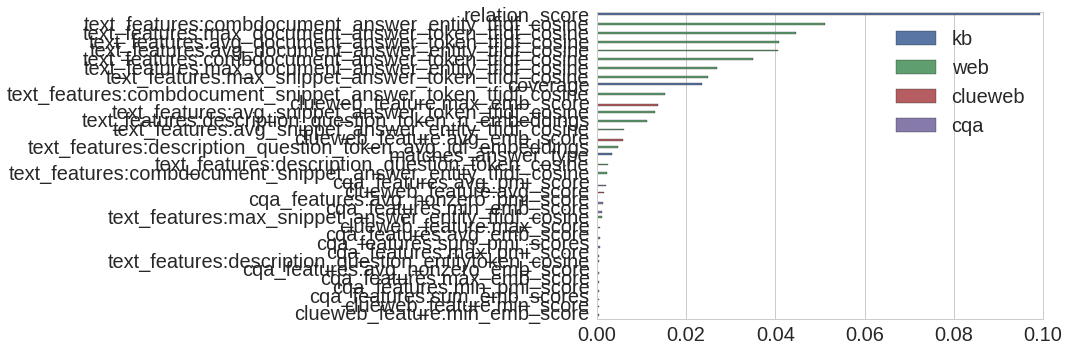
\includegraphics[width=0.8\textwidth]{img/feature_importances}
\vspace{-4mm}
\caption{A plot of Gini importances of different features of our answer ranking random forest model (features marked * are not text-based and are provided for comparison)}
\label{fig:feature_importances}
\end{figure*}

In summary, Text2KB significantly outperforms the baseline system, and each of the introduced components contributes to this improvement.
Web search results data turned out to be the most useful resource, and it significantly improves the quality by helping with question entity identification and candidate ranking.
Next, we analyze the system performance in more detail, and investigate factors for future extension.